% !TeX spellcheck = ca
\documentclass{article}
\usepackage[utf8]{inputenc}
\usepackage{amsmath}
\usepackage{ amssymb }
\usepackage{float}
\usepackage{graphicx}

%Tot això hauria d'anar en un pkg, però no sé com és fa
\newcommand*{\assignatura}[1]{\gdef\1assignatura{#1}}
\newcommand*{\grup}[1]{\gdef\3grup{#1}}
\newcommand*{\professorat}[1]{\gdef\4professorat{#1}}
\renewcommand{\title}[1]{\gdef\5title{#1}}
\renewcommand{\author}[1]{\gdef\6author{#1}}
\renewcommand{\date}[1]{\gdef\7date{#1}}
\renewcommand{\baselinestretch}{1.5}
\renewcommand{\maketitle}{ %fa el maketitle de nou
	\begin{titlepage}
		\raggedright{UNIVERSITAT DE LLEIDA \\
			Escola Politècnica Superior \\
			Grau en Enginyeria Informàtica\\
			\1assignatura\\}
		\vspace{5cm}
		\centering\huge{\5title \\}
		\vspace{3cm}
		\large{\6author} \\
		\normalsize{\3grup}
		\vfill
		Professorat : \4professorat \\
		Data : \7date
\end{titlepage}}
%Emplenar a partir d'aquí per a fer el títol : no se com es fa el package
%S'han de renombrar totes, inclús date, si un camp es deixa en blanc no apareix


\title{Práctica de Modelos Probabilísticos - Predicción dela valoración de alojamientos de AirBnB}
\author{Joaquim Picó Mora, Ian Palacín Aliana}
\date{Dilluns 8 Juny}
\assignatura{Aprenentatge i Raonament Automàtic}
\professorat{R.Bejar}
\grup{}

\renewcommand{\refname}{Bibliografia}

%Comença el document
\begin{document}
	\maketitle
	\thispagestyle{empty}


\section{Generador de arff}	
% Explicació de com executar l'script
L'script està realitzat amb python 3, així que una forma d'executar-lo és fent:
\begin{verbatim}
python3 generate_arff.py <data-set> <out-learning-dataset> <out-evaluation-dataset>
\end{verbatim}
També es pot executar donant permisos al fitxer python mitjançant:
\begin{verbatim}
chmod +x  generate_arff.py
./generate_arff.py <data-set> <out-learning-dataset> <out-evaluation-dataset>
\end{verbatim}
On $<data-set>$ és el nom del data set d'entrada, en el nostre cas barca.csv, i $<out-learning-dataset>$ i $<out-evaluation-dataset>$ són el nom dels fitxers de sortida traduits a arff per a l'aprenentatge i l'avaluació de la xarxa.\\
A l'executar l'script, si no es fica el nombre d'arguments que és demana s'imprimeix un missatge amb el mètode d'ús i es surt del programa. 
\section{Puntuación de los modelos}
% Puntuació log(UPSM) i error de classificació  de tots els models
% de tots els models
\subsection{Classe 1}
\begin{table}[H]
\begin{tabular}{ll}
\hline
Error classificació & log(UPSM)           \\
\hline
48.6863 \%          & -103784.93516475169 \\
48.6863 \%          & -103845.33539207192 \\
48.9079 \%          & -103702.10859464137 \\
48.8762 \%          & -103940.05807545574 \\
48.8762 \%          & -103865.53730402223 \\
48.6863 \%          & -103799.35937336765 \\
48.8762 \%          & -104599.69306872078 \\
48.8762 \%          & -103840.89609789594 \\
48.9079 \%          & -103833.55088340564 \\
48.8762 \%          & -103892.78517133751
\end{tabular}
\end{table}
\subsection{Classe 2}
\begin{table}[H]
\begin{tabular}{ll}
\hline
Error classificació & log(UPSM)           \\
\hline
50.1108 \%          & -127916.12156930043
\end{tabular}
\end{table}
\subsection{Classe 3}
\begin{table}[H]
\begin{tabular}{ll}
\hline
Error classificació & log(UPSM)           \\
\hline
48.528  \%          & -105938.04552255767 \\
48.5597 \%          & -105871.05201856224 \\
49.0028 \%          & -106280.47076199797 \\
48.9712 \%          & -105640.32391213975 \\
48.1798 \%          & -105671.92496621847 \\
47.9899 \%          & -105982.94208430553 \\
49.446  \%          & -105844.14592852714 \\
48.2431 \%          & -105889.99653741406 \\
48.4014 \%          & -106654.81244066187 \\
48.6863 \%          & -105914.39769708786
\end{tabular}
\end{table}
\section{Mejor modelo}
\subsection{Clase 1}
En aquest cas el millor model és el primer que apareix a la taula. Tot i que veiem que hi ha dos altres models que tenen el mateix percentatge d'error de classificació, el que resulta tenir el UPSM score més alt és el primer model.
\begin{figure}[H]
  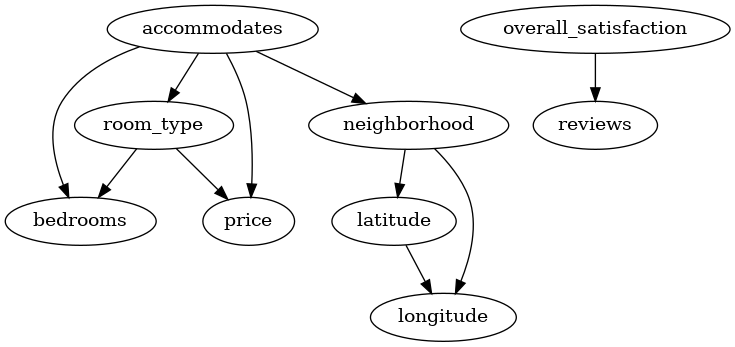
\includegraphics[width=\linewidth]{classe1.png}
  \caption{Graph xarxa classe 1.}
  \label{fig:gp1}
\end{figure}
\subsection{Clase 2}
\begin{figure}[H]
  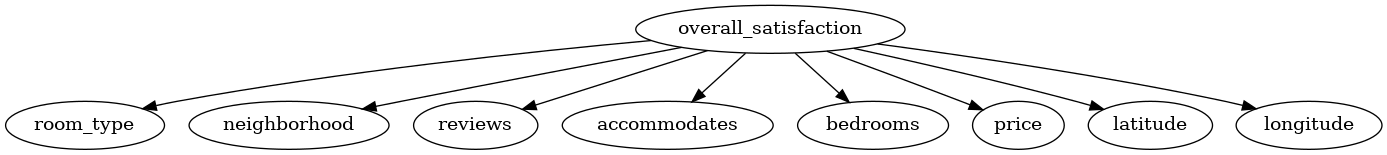
\includegraphics[width=\linewidth]{classe2.png}
  \caption{Graph xarxa classe 2.}
  \label{fig:gp2}
\end{figure}
\subsection{Clase 3}
Aquí es veu mes clar que el millor model és el sisé que apareix en la taula, ja que és el que té el percentatge d'errors més baix.
\begin{figure}[H]
  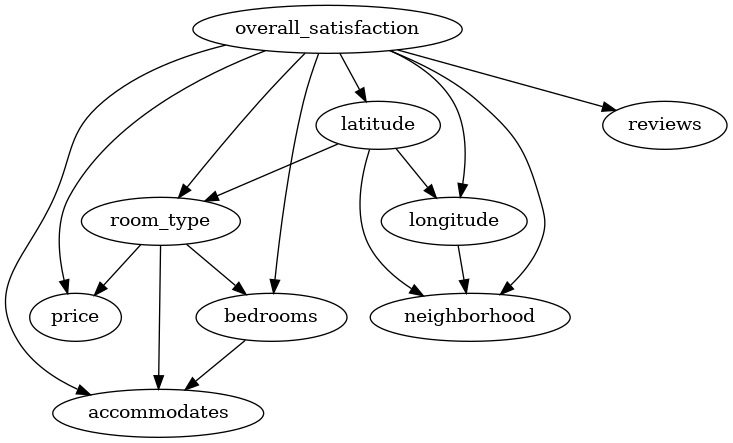
\includegraphics[width=\linewidth]{classe3.png}
  \caption{Graph xarxa classe 3.}
  \label{fig:gp3}
\end{figure}

\section{Justificación tamaño}
%Primer vam provar sense cap tipus de reducció
%Després vam probar a reduir latitut i longitud ja que era el camp que més valors diferents. Ho vam fer per quartils.
%Després també ens en vam adonar de que podiam reduir el preu i les reviews ja que eren camps quantitatius i per tant reductibles. Els vam "agrupar" de 20 en 20.
%Per overall satisfaction vam decidir canviar els simbols
%Podria ser que al haver tants valors diferents la xarxa entrenada acabes tenint molt overfeating.
\end{document}